\documentclass[10pt,aspectratio=43]{beamer}
%\usepackage{nju}			 %导入 nju 模板宏包
%\usepackage[UTF8]{ctex}      %导入 ctex 宏包,添加中文支持
\usepackage{xeCJK}
\usepackage{amsmath,amsfonts,amssymb,bm}   %导入数学公式所需宏包
\usepackage{color}			 %字体颜色支持
\usepackage{graphicx,hyperref,url}
\usepackage{listings}
\usepackage{booktabs}
\usepackage{multirow}
\usepackage{float}
\usepackage{mhchem}
\usepackage{animate}
\usepackage[isbn=false,doi=false,url=false,uniquename=init,style=chem-acs]{biblatex}
\addbibresource{icc_pre_1108.bib}
\AtEveryCitekey{\clearfield{title}}
\AtEveryBibitem{\clearfield{title}}
\usepackage{textcomp}
\usepackage{multicol}

\usepackage{listings}
\definecolor{dkgreen}{rgb}{0,0.6,0}
\definecolor{gray}{rgb}{0.5,0.5,0.5}
\definecolor{mauve}{rgb}{0.58,0,0.82}
\lstset{ %
	language=Python,                % the language of the code
	basicstyle=\Consolas\footnotesize,           % the size of the fonts that are used for the code
	numbers=left,                   % where to put the line-numbers
	numberstyle=\tiny\color{gray},  % the style that is used for the line-numbers
	stepnumber=1,                   % the step between two line-numbers. If it's 1, each line 
	% will be numbered
	numbersep=5pt,                  % how far the line-numbers are from the code
	backgroundcolor=\color{white},      % choose the background color. You must add \usepackage{color}
	showspaces=false,               % show spaces adding particular underscores
	showstringspaces=false,         % underline spaces within strings
	showtabs=false,                 % show tabs within strings adding particular underscores
	frame=single,                   % adds a frame around the code
	rulecolor=\color{black},        % if not set, the frame-color may be changed on line-breaks within not-black text (e.g. commens (green here))
	tabsize=4,                      % sets default tabsize to 2 spaces
	captionpos=b,                   % sets the caption-position to bottom
	breaklines=true,                % sets automatic line breaking
	breakatwhitespace=false,        % sets if automatic breaks should only happen at whitespace
	title=\lstname,                   % show the filename of files included with \lstinputlisting;
	% also try caption instead of title
	keywordstyle=\color{blue},          % keyword style
	commentstyle=\color{dkgreen},       % comment style
	stringstyle=\color{mauve},         % string literal style
	escapeinside={\%*}{*)},            % if you want to add LaTeX within your code
	morekeywords={*,...}               % if you want to add more keywords to the set
}
\usepackage{multicol}
\usepackage{multirow}
\usepackage{siunitx}
\definecolor{codegray}{gray}{0.9}
\newfontfamily\Consolas{Consolas}
\newcommand{\code}[1]{\colorbox{codegray}{{\Consolas#1}}}
\newcommand{\hl}[1]{\colorbox{yellow}{#1}}
\lstnewenvironment{mcode}
{\lstset{backgroundcolor=\color{lightgray},
		xleftmargin=0.5cm,
		frame=tlbr,framesep=4pt,framerule=0pt,
		%language=python,
		keepspaces=false,
		numbers=none
}}%
{}

\usepackage{tikz,mathpazo}
\usetikzlibrary{shapes.geometric, arrows}
\usetikzlibrary{calc}
\tikzstyle{box} = [rectangle, minimum width = 1.5cm, minimum height=0.8cm,text centered, draw = black]
\tikzstyle{rbox} = [rectangle, rounded corners, minimum width = 1.5cm, minimum height=0.8cm,text centered, draw = black, fill = blue!40]
\tikzstyle{arrow} = [->,>=stealth]

%\beamertemplateballitem		%设置 Beamer 主题
%\catcode`\。=\active        %或者=13
%\newcommand{。}{.}         %将正文中的“。”号转换为“.”。

%\AtBeginSection[]
%{
%  \begin{frame}
%    \frametitle{Contents}
%    \tableofcontents[currentsection]
%  \end{frame}
%}



\title{Orbitals: Population Analysis, Transformation and Visualization}	        %首页信息设置

\author[]{            %个人信息设置
    Shirong Wang\\[0.3cm]
    %15XXXXXXXX\\[0.3cm]
    Kuang Yaming Honors School}

\date{\today}



\begin{document}

% 参与反应的轨道
% Pt,Pd,Ni,P
% 不同构象NBO
% Me->H,CF3

\begin{frame}
\hfill ICC Report III
\titlepage
\end{frame}

\begin{frame}
\frametitle{Contents}
\tableofcontents
\end{frame}

\section{Population Analysis}
\begin{frame}
\frametitle{Atomic Charges}
\begin{enumerate}
	\item Wavefunction-based (aka population analysis)
	\item Real-space-based
	\item Electrostatic-potential-based
\end{enumerate}
\end{frame}

\begin{frame}
\frametitle{Wavefunction-based Atomic Charges}
\begin{itemize}
	\item Mulliken charges, L\"owdin charges
	\item NPA charges\\
	\code{pop=nbo}
\end{itemize}

\end{frame}

\begin{frame}
\frametitle{Real-space-based Atomic Charges}
\begin{itemize}
	\item Hirshfeld charges
	\item Becke charges
	\item AIM charges
\end{itemize}
\end{frame}

%\begin{frame}
%\frametitle{Electrostatic-potential-based Atomic Charges}
%\begin{itemize}
%	\item MK
%	\item CHelpG
%\end{itemize}
%\end{frame}

\section{Molecular Orbitals}
\begin{frame}
\frametitle{Natural Bonding Orbitals}
PNAO -- NAO -- NHO -- NBO -- NLMO
\end{frame}
\defverbatim[colored]\makeset{
\begin{mcode}
#p B3LYP/6-31G(d,p) Pop=NBORead 

Example of NBO bond orders

0  1
C     0.000000    0.665676    0.000000
H     0.919278    1.237739    0.000000

$nbo $end


\end{mcode}
}
\begin{frame}
\frametitle{NBO Technical Details}
\textbf{Run NBO3.1 via Gaussian}
\makeset
\textbf{Run NBO6/7}~\\
\code{\$nbo archive file=... \$end}

\begin{figure}
	\centering
	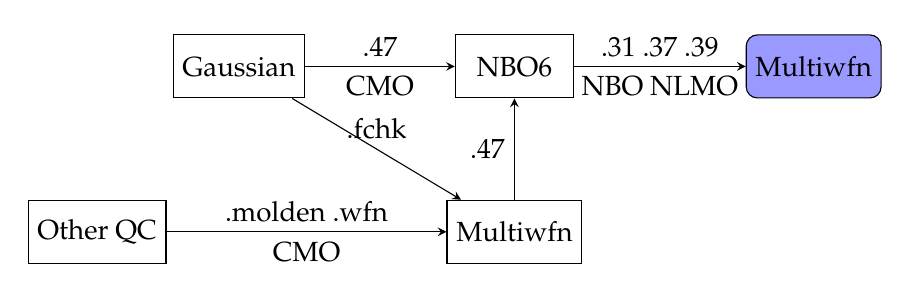
\begin{tikzpicture}[node distance=1.5cm]
	\node (G) [box] {Gaussian};
	\node (M1) [box, right of=G, xshift=2cm, below of=G, yshift=-0.6cm] {Multiwfn};
	\node (NBO6) [box, right of=G, xshift=2cm] {NBO6};
	\node (M) [rbox, right of=NBO6, xshift=2.3cm] {Multiwfn};
	\node (Other) [box, below of=G, yshift=-0.6cm, left of=G, xshift=-0.3cm]{Other QC};
	%\draw [arrow](G) -- node[anchor=south]{.fchk} (M);
	\draw [arrow](G) -- node[anchor=south]{.47} node[anchor=north]{CMO} (NBO6);
	\draw [arrow](G) -- node [anchor=south]{.fchk} (M1);
	\draw [arrow](Other) -- node [anchor=south]{.molden .wfn} node[anchor=north]{CMO} (M1);
	\draw [arrow](M1) -- node[anchor=east]{.47} (NBO6);
	\draw [arrow](NBO6) -- node[anchor=south]{.31 .37 .39} node[anchor=north]{NBO NLMO} (M);
	\end{tikzpicture}
	%\caption{\label{fig: }}
\end{figure}
\end{frame}

\defverbatim[colored]\makeset{
\begin{mcode}
$CHOOSE 
BOND S 1 28
     S 1 29 END
3CBOND S 1 28 29 END
$END			
\end{mcode}
}
\begin{frame}
Useful NBO keywords
\begin{itemize}
	\item \code{\$NBO NLMO PLOT \$END}
	\item user-defined search.
	\begin{itemize}
		\item NBO6\\
        \makeset
		%\code{\$CHOOSE BOND S 1 28 END \$END}\\
		%\code{\$CHOOSE 3CBOND S 1 28 29 END \$END}
		\item NBO7\\
		\code{\$NBO MOLUNIT <1,28,29> \$END} 
	\end{itemize}
\end{itemize}
\end{frame}

\begin{frame}
\frametitle{Orbital Localization}
\begin{figure}
	\centering
	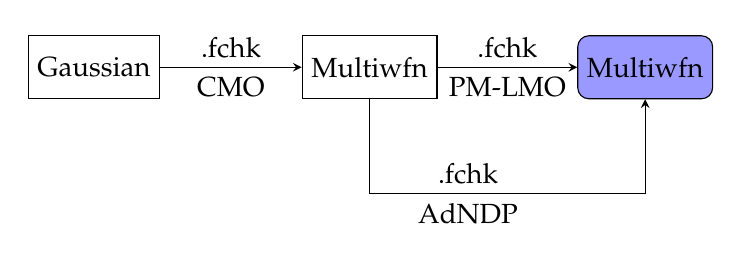
\begin{tikzpicture}[node distance=1.5cm]
	\node (G) [box] {Gaussian};
	\node (M) [box, right of=G, xshift=2cm] {Multiwfn};
	%\node (NBO6) [box, right of=G, xshift=2cm] {NBO6};
	\node (MV) [rbox, right of=M, xshift=2cm] {Multiwfn};
	%\draw [arrow](G) -- node[anchor=south]{.fchk} (M);
	\draw [arrow](G) -- node[anchor=south]{.fchk} node[anchor=north]{CMO} (M);
	\draw [arrow](M) -- node[anchor=south]{.fchk} node[anchor=north]{PM-LMO} (MV);
	\draw [arrow](M) -- ($(M.south) + (0,-1.2)$) -- node[anchor=south]{.fchk} node[anchor=north]{AdNDP} ($(M.south) + (2.5,-1.2)$) -| (MV);
	\end{tikzpicture} 
	%\caption{\label{fig: }}
\end{figure}

\end{frame}




\end{document}